\documentclass[conference]{IEEEtran}

%+++++++++++++++++++++++++++++++++++++++++++++++++++
\usepackage[pdftex]{graphicx}
\usepackage{amsmath}
\usepackage{eqparbox}
\usepackage{amsmath, amssymb}
\usepackage[hidelinks]{hyperref}
\usepackage{float}
%+++++++++++++++++++++++++++++++++++++++++++++++++++


\hyphenation{op-tical net-works semi-conduc-tor IEEEtran}
\begin{document}

%+++++++++++++++++++++++++++++++++++++++++++++++++++
\title{\LARGE Social Network Community Detection} 
\author{Alua Tursynkhan, Anel Kim, Meirzhan Kurmanov, Zhanel Yerzhanova, Madi Skakov}

%+++++++++++++++++++++++++++++++++++++++++++++++++++

\maketitle


\begin{abstract}
    We apply community detection algorithms to analyze political divisions using the 2004 Amazon political books dataset. By representing books as nodes and frequent co-purchases as edges, we identify clusters of liberal, conservative, and neutral books. We compare the standard k-means algorithm with the method of Lancichinetti et al., discussing their strengths and limitations. Our results show how network analysis can reveal societal polarization and improve recommendation systems and policy decisions.
\end{abstract}


\section{INTRODUCTION}

Networks and communities are one of the most fundamental things we deal with in daily life. These are very interesting structures to study and analyzing them can provide us with valuable information that can be used to solve real world problems.

In social networks, individuals are represented as nodes and their interactions as edges. This network representation allows community detection algorithms to be effectively applied to reveal community structures within such systems \cite{malode2025comparative}. Community detection is the process of identifying groups of interacting nodes in a network based on their structural properties. These algorithms analyze how nodes are interconnected to identify hidden structures or communities \cite{Li2016CDAB}

One of many examples of useful application of network analysis is detection of cartels in auction bidding in the research done by Wachs and Kertesz \cite{wachs2019network}. By drawing the edges between the participants with "unusual" co-bidding behavior and applying community detection algorithms, they were able to detect an existing cartel in the Ohio public school milk supply contract.

So, we decided to apply the network approach to find a solution to our own problem, analyzing political division is society through the sales in the Amazon book store of political literature. 2004 political books dataset\cite{newman_netdata}, a network with nodes representing books about US politics and Edges between books show frequent co-purchasing of those books by the same buyers on Amazon. By applying community detection algorithms, we identified three distinct clusters: liberal, conservative, and neutral books. This clustering transforms the raw dataset into a useful instrument for examining societal political division. These insights have real-world applications: enhancing recommendation systems, encouraging inter-ideological discussion, and assisting in the formulation of polarization and media literacy policy decisions. Therefore, community detection aids in comprehending the dynamics of society as a whole.

This paper discusses the classical \textit{k}-means algorithm and the method proposed by Lancichinetti et al. \cite{lancichinetti2009detecting} in the context of community detection in social networks. The advantages and limitations of each approach are examined, and a solution to our problem using these algorithms is presented.

\section{K-Means Clustering}

Clustering groups data points, placing those with the highest similarity into the same cluster and separating them from points that are less alike \cite{anderberg1973cluster}. Similarity can be measured using metrics such as Manhattan distance, Minkowski distance, or cosine similarity \cite{irani2016clustering}.

\textit{K}-means clustering is one of the most popular clustering algorithms due to its simplicity and efficiency \cite{slonim2013hartigan}. It is an unsupervised machine learning algorithm that partitions a dataset into $K$ distinct, non-overlapping clusters. Traditionally, it uses the Euclidean distance as a metric to identify similarities between data points \cite{irani2016clustering}. However, the method is sensitive to outliers and noise in the dataset \cite{yu2018two}.

In this paper, we focus on Lloyd's algorithm, also known as the batch version of k-means.

\subsection*{Algorithm}

The standard \textit{k}-means algorithm, proposed by Stuart Lloyd in 1957 \cite{lloyd1982least}, partitions a dataset ${X} = \{x_1, \ldots, x_n\} \subset \mathbb{R}^m$ into $K$ clusters $\{C_1, \ldots, C_K\}$ by minimizing the mean distortion, which measures how well the data points fit the assigned clusters.

The distortion function $D$ is defined as:
\begin{equation}
    D(C) = \frac{1}{n}\sum_{k=1}^K \sum_{x_i \in C_k} \|x_i - \mu_k\|^2
\end{equation}
where: 
\begin{itemize}
    \item $n$ – total number of data points,
    \item $\mu_k$ – the centroid of cluster $C_k$,
    \item $\|.\|^2$ – squared Euclidean distance.
\end{itemize}

The algorithm consists of three main steps: initialization, assignment (E-step), and update (M-step).
\begin{enumerate}
    \item \textit{Initialization:} $K$ centroids $\mu_k$ are randomly chosen, either uniformly at random or using advanced methods like k-means++.
    \item \textit{Assignment:} Each data point $x_i \in X$ is assigned to the nearest cluster based on Euclidean distance:
    \begin{equation}
        z_i = \arg\min_{k \in \{1, \dots, K\}} \left\| x_i - \mu_k \right\|^2
    \end{equation}
    \item \textit{Update:} Each centroid $\mu_k$ is updated as the mean of all points assigned to cluster $C_k$:
    \begin{equation}
        \mu_k = \frac{1}{\left| C_k \right|} \sum_{x_i \in C_k} x_i
    \end{equation}
\end{enumerate}

These steps are repeated until convergence. In Lloyd’s algorithm, all data points are reassigned before centroids are updated — hence the term \textit{batch} update \cite{slonim2013hartigan}\cite{lloyd1982least}.

\subsection*{K-Means for Social Network Community Detection}
Among traditional community detection algorithms, \textit{k}-means is a widely used method for partition clustering \cite{JAVED201887}. However, since \textit{k}-means relies on Euclidean distance to group items into clusters, it is not directly applicable to raw network graph data, where nodes are connected by edges rather than existing in a continuous vector space. 

In our paper, we focus on applying standard \textit{k}-means. To make this possible for graph data, we first represent each node as a numerical feature vector. Specifically, we extract three structural features from each node: degree, clustering coefficient, and betweenness centrality\cite{dacunha2025identify}.
\begin{itemize}
    \item The degree of each node is the number of its neighbors.
    \item The local clustering coefficient C of a node v examines the existing connections between its neighboring nodes. It is calculated as follows:
    \begin{equation}
        C_v = \frac{2T_v}{k_v(k_v-1)}
    \end{equation}
    where:
    \begin{itemize}
        \item $T_v$ - the number of connected pairs of neighbors of v;
        \item $k_v$ - degree of node v;
    \end{itemize}
    \item The betweenness centrality is a measure of how often a node lies in the shortest paths between other nodes:
    \begin{equation}
        C_B(v)= \sum_{s\neq v\neq e} \frac{\sigma_{se}(v)}{\sigma_{se}}
    \end{equation}
    where:
    \begin{itemize}
        \item $s, e$ - starting and ending nodes;
        \item $\sigma_{se}(v)$ - the number of those shortest paths that pass through node v;
        \item $\sigma_{se}$ - total number of shortest paths from node s to node e;
    \end{itemize}
\end{itemize}

Once each node is embedded in this 3-dimensional feature space, we can apply \textit{k}-means clustering to detect communities within the network.

However, despite these enhancements, most \textit{k}-means-based algorithms are not well-suited for detecting overlapping community structures in large-scale social networks. This limitation arises because \textit{k}-means is inherently designed to assign each data point to exactly one cluster \cite{JAVED201887}\cite{Li2016CDAB}\cite{malode2025comparative}. As a result, alternative methods that can handle overlapping structures may be more suitable for such tasks.

\section{Lancichinetti et al. (2009) method}
The method we use is based on the article \cite{lancichinetti2009detecting}, with the main focus on the optimization of the fitness function. In terms of community detection, a \textbf{fitness function} is a measurable method that assesses the quality of a provided partition of the network into communities. The partition is defined as a special way of distributing the nodes of a network (or graph) into disjoint subsets, where each subset is called a community. The main problem we are trying to work out here is the overlapping communities, which means that the nodes can belong to more than one community at the same time. This is also noticed in the real world, since many nodes naturally are in multiple groups at once. These nodes are, most of the time, a problem for the standard methods and lead to misclassifications. Our method considers this issue and introduces a local exploration of the network, which in turn will detect the natural community of each node. 

\subsection*{Algorithm}
The algorithm's main aim is to detect overlapping communities.  The main idea behind our algorithm is that communities are made up of nearby nodes. A community is found by finding a group of nodes with the highest measure of a certain feature. The fitness function is identified as:
\begin{equation}
    f_{\mathcal{G}} = \frac{k_{\text{in}}^{\mathcal{G}}}{\left(k_{\text{in}}^{\mathcal{G}} +k_{\text{out}}^{\mathcal{G}}\right)^\alpha}
\end{equation}
where:
\begin{itemize}
    \item \( k_{\text{in}}^{\mathcal{G}} \) is the total internal degree of the nodes of cluster \( \mathcal{G} \), equal to twice the number of internal links within the cluster, 
    \item \( k_{\text{out}}^{\mathcal{G}} \) is the total external degree of the nodes of cluster \( \mathcal{G} \), defined as the number of links connecting cluster with the rest of the graph, 
    \item \( \alpha \) is a positive parameter that controls the size of the communities.
\end{itemize}

The formula above finds the fitness of a cluster (module). Now, we introduce a formula for calculating the fitness of a single node. The node fitness is the concept that measures a single node's contribution to a subgraph's overall fitness function. It is defined as: 
\begin{equation}
    f_{\mathcal{G}}^{A} = f_{\mathcal{G} + \{A\}} - f_{\mathcal{G} - \{A\}}
\end{equation}
where \( f_{\mathcal{G}}^{A} \) is the fitness of node A with respect to subgraph $\mathcal{G}$, i.e.
\begin{itemize}
    \item \( \mathcal{G} + \{A\} \) denotes the subgraph obtained from module \(\mathcal{G}\) with node \textit{A}, 
    \item \( \mathcal{G} - \{A\} \) denotes the subgraph obtained from module \(\mathcal{G}\) without node \textit{A}. 
\end{itemize}

Let us assume that we select a subgraph $\mathcal{G}$ that contains node $A$ as one of its members. In the beginning,  the subgraph \(\mathcal{G}\) is classified with only node \textit{A}, $k_{\text{in}}^{\mathcal{G}}$ = 0. To find the  \textit{natural community} of node A, we perform the following steps:
\begin{enumerate}
    \item Calculate the fitness function of all the neighboring nodes of $\mathcal{G} $ that are not included in $\mathcal{G}$; 
    \item The neighbor with the largest fitness is added to \( \mathcal{G}\), which in turn results in a new, bigger subgraph \( \mathcal{G}'\);
    \item Recalculate the fitness of each node of \( \mathcal{G}'\);
    \item If any node has a negative fitness value, remove it from \( \mathcal{G}'\) and that results in producing a new subgraph \( \mathcal{G}''\);
    \item If step 4 occurs, repeat from step 3; in other cases, repeat from 1 for the subgraph \( \mathcal{G}''\).
\end{enumerate}

\begin{figure}[ht]
  \centering
  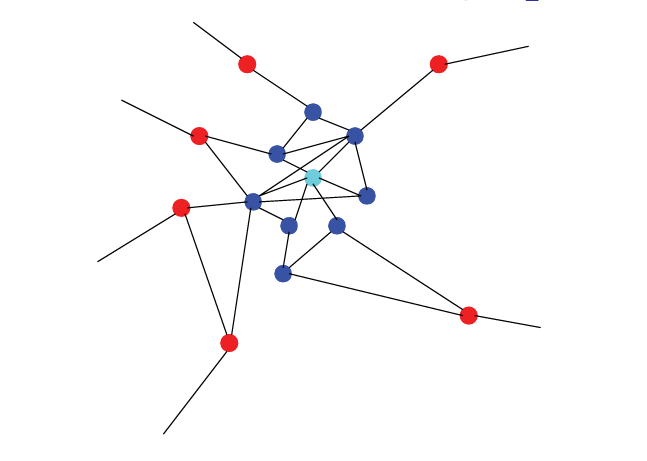
\includegraphics[width=0.5\textwidth]{fig1_network_image.png}
  \caption{The sample of natural community for a node (sky-blue point). The blue nodes are the other community members and have positive fitness, meanwhile red dots all have negative fitness \cite{lancichinetti2009detecting}.}
  
\end{figure}


This algorithm stops when all the nodes in step 1 have negative fitness. 

The \textit{cover} of the graph is defined as a distribution of communities (clusters) such that each node is assigned to at least one community (cluster). The cover lets us see the overlapping communities. However, in our case, finding the cover of the graph would be computationally expensive, as that means that we have to perform the algorithm written above for each node. Many nodes' natural communities would be the same, and we would have to spend most of our time identifying the same groups again and again. For that reason, we prefer to use a more computationally feasible algorithm:
\begin{enumerate}
    \item Pick a node \textit{A} at random;
    \item Detect the natural community of \textit{A};
    \item Select at random a node \textit{B} that is not yet assigned to any group;
    \item Detect the natural community of node \textit{B} by considering all the nodes without their possible membership to other groups;
    \item Repeat from 3.
\end{enumerate}
This algorithm stops when all nodes have been assigned to at least one group.

Changing the parameter \( \alpha \) allows us to change the resolution of communities; for example, large values of \( \alpha \) separate the graph into very small communities, while small values group nodes in large groups. The best choice would be \( \alpha \) = 1, since it gives enough information about the community structure of the graph. If we use a fixed value for \( \alpha \), it limits the resolution at which the method can detect communities. However, we do not know how large or small the communities are beforehand, so it is significant to compare the covers obtained at different scales. Each \( \alpha \) may produce a different cover. Nevertheless, there are certain ranges for \( \alpha \) such that the cover stays the same. A stable cover is expected to remain across a wide range of \( \alpha \) values, representing stability. To evaluate and classify a cover \( \mathcal{P}\) quantitatively, the authors introduce an index: the \textit{average fitness} of its communities. This is computed by averaging the fitness values \(f_\mathcal{G_i}\) of all communities in the cover when \( \alpha = 1\):
\begin{equation}
    \bar{f}_{\mathcal{P}} = \frac{1}{n_c} \sum_{i=1}^{n_c} f_{\mathcal{G}_i} \quad (\alpha = 1)
\end{equation}
where:
\begin{itemize}
    \item \( \bar{f}_{\mathcal{P}} \) is the average fitness of the cover,
    \item \( n_c \) is the number of communities in the cover \( \mathcal{P} \),
    \item \( f_{\mathcal{G}_i} \) is the fitness of the \( i \)-th community in the cover.
\end{itemize}


\section{Datasets}
The testing of both algorithms was achieved using sample datasets and a problem dataset. For sample datasets we picked "Zachary's Karate Club" and "Dolphin Social Network". As for the problem dataset, we picked "Books about US politics" which was mentioned earlier. All three of them were open-source which made it possible to easily obtain those datasets \cite{newman_netdata}. They are unweighted, undirected graphs which are perfectly suitable for evaluating algorithms that we chose.
\subsection{Karate club}
This dataset represents the social network of friendships between 34 members of a karate club at a US university, as observed by Wayne Zachary in the 1970s. Each node corresponds to a member, and edges represent social interactions. The network is notable for its clear community structure, especially following a split of the club into two factions \cite{newman_netdata}.
\subsection{Dolphins}
This network captures the social interactions among 62 bottlenose dolphins living off the coast of New Zealand. Nodes represent individual dolphins, and edges represent frequent association between pairs. The network naturally exhibits community divisions, making it an excellent benchmark for community detection methods. For our algorithms, we chose to use the dolphins’ gender as the ground-truth community division. This allowed us to evaluate the algorithm’s ability to detect natural groupings based on biological and social factors \cite{newman_netdata}.
\subsection{Books about US politics}
This dataset includes books about US politics sold by Amazon.com around the 2004 presidential election. Nodes represent books, and edges indicate frequent co-purchasing by the same buyers. Books are labeled as liberal, conservative, or neutral, allowing for a ground-truth community structure useful for validation \cite{newman_netdata}.

\section{Results' Analysis}
To analyze the results of each algorithm, we decided to use Overlapping Normalized Mutual Information, a metric applied to compare the similarity between two overlapping community structures in graphs such as the ground truth communities and those detected by our algorithms\cite{lancichinetti2009detecting}. The reason we used this metric is that ONMI can consider the mixed cases with non-overlapping truth but the algorithm detects overlapping communities. In addition, via entropy and conditional entropy it measures how much the detected community membership structure captures the true structure, not just overlaps. 







Each node can belong to multiple communities. For every node \( i \):
\begin{itemize}
    \item \( X_i \) is the set of ground truth communities that node \( i \) belongs to
    \item \( Y_i \) is the set of detected communities that node \( i \) belongs to
\end{itemize}

\subsection*{Entropy of Each Assignment}

Entropy shows how spread out the community assignment is \cite{cover2006}.



Let:
\begin{itemize}
    \item \( C_X \) be the set of all ground truth communities
    \item \( N \) be the total number of nodes
\end{itemize}

For each community \( c \in C_X \), define:

\[
P(c) = \frac{\text{number of nodes in } c}{N}
\]

Then, the entropy of the ground truth is given as:

\[
H(X) = -\sum_{c \in C_X} P(c) \log P(c)
\]

Similarly, for detected communities \( C_Y \):

\[
H(Y) = -\sum_{k \in C_Y} P(k) \log P(k)
\]
where:

\[
P(k) = \frac{\text{number of nodes in } k}{N}
\]

\subsection*{Conditional Entropy}

Conditional entropy refers to how well one set of communities can predict another \cite{cover2006}.

For each pair \( (c, k) \) where:
\begin{itemize}
    \item \( c \in C_X \): a ground truth community
    \item \( k \in C_Y \): a detected community
\end{itemize}

Define:
\begin{itemize}
    \item \( n_{11} \): number of nodes in both \( c \) and \( k \)
    \item \( n_{10} \): number of nodes in \( c \) but not in \( k \)
    \item \( n_{01} \): number of nodes in \( k \) but not in \( c \)
    \item \( n_{00} \): number of nodes in neither \( c \) nor \( k \)
\end{itemize}

Let \( N \) be the total number of nodes.

The conditional entropy of community \( c \) given community \( k \) is \cite{cover2006}:

\[
H(c \mid k) = -\sum_{a,b \in \{0,1\}} \frac{n_{ab}}{N} \log \left( \frac{n_{ab}/N}{(n_{a0}+n_{a1})/N} \right)
\]

In other words, H measures how much uncertainty is left about \( c \) when we know \( k \).

Then, for the whole ground truth community c we should find the matching community k that gives the lowest conditional entropy and find their sum:

\[
H(X \mid Y) = \sum_{c \in C_X} \min_{k \in C_Y} H(c \mid k)
\]

Similarly:

\[
H(Y \mid X) = \sum_{k \in C_Y} \min_{c \in C_X} H(k \mid c)
\]

\subsection*{Mutual Information}

The mutual information is:

\[
MI(X,Y) = H(X) - H(X \mid Y)
\]

\[
MI(Y,X) = H(Y) - H(Y \mid X)
\]
It assesses the extent to which understanding the identified communities lowers uncertainty about the ground truth communities (and vice versa) \cite{mutual}.
\subsection*{ONMI Formula}

The final Overlapping Normalized Mutual Information is given \cite{lancichinetti2009detecting}\cite{mutual}:

\[
ONMI(X,Y) = \frac{1}{2} \left( \frac{MI(X,Y)}{H(X)} + \frac{MI(Y,X)}{H(Y)} \right)
\]


\subsection*{Interpretation of the results}

For each of the datasets (Zachary's Karate Club, Dolphin School network, Political literature network), we obtained the following metrics: 

\begin{table}[ht]
\centering
\begin{tabular}{|c|c|c|c|}
\hline
          & Z. K. C. & Dolphin School & Political literature \\
\hline
K-means (NMI)    & 0.0062 & 0.0153 & 0.0189 \\
Lancichinetti  (ONMI)   & 0.6905 & 0.8768 & 0.4338 \\
\hline
\end{tabular}
\caption{The values of the metics}
\end{table}

The results suggest that algorithm proposed by Lancichinetti performed far better than K-means. Since for Lancichinetti algorithm, these values of ONMI score were obtained by varying parameters of $\alpha$, we chose those parameters, where the score peaked the highest. Namely, 
\begin{itemize}
    \item Z.K.C. ($\alpha \in \{ 0.8, 0.81, 0.82, 0.83\}$)
    \item Dolphin School ($\alpha \in \{0.825, 0.83\}$)
    \item Political Literature ($\alpha = 0.77$)
\end{itemize}

\subsection*{Visual results of algorithms}
\subsection{K-means clustering}
The following is a representation of the ground-truth graphs and the graphs labeled after clustering of K-means. 
The visualization highlights the alignment and discrepancies between the ground truth and an algorithmic output. 
The K-means algorithm attempts to group nodes based on similarity, without direct knowledge of the original community structures. 

\begin{figure}[H]
  \centering
  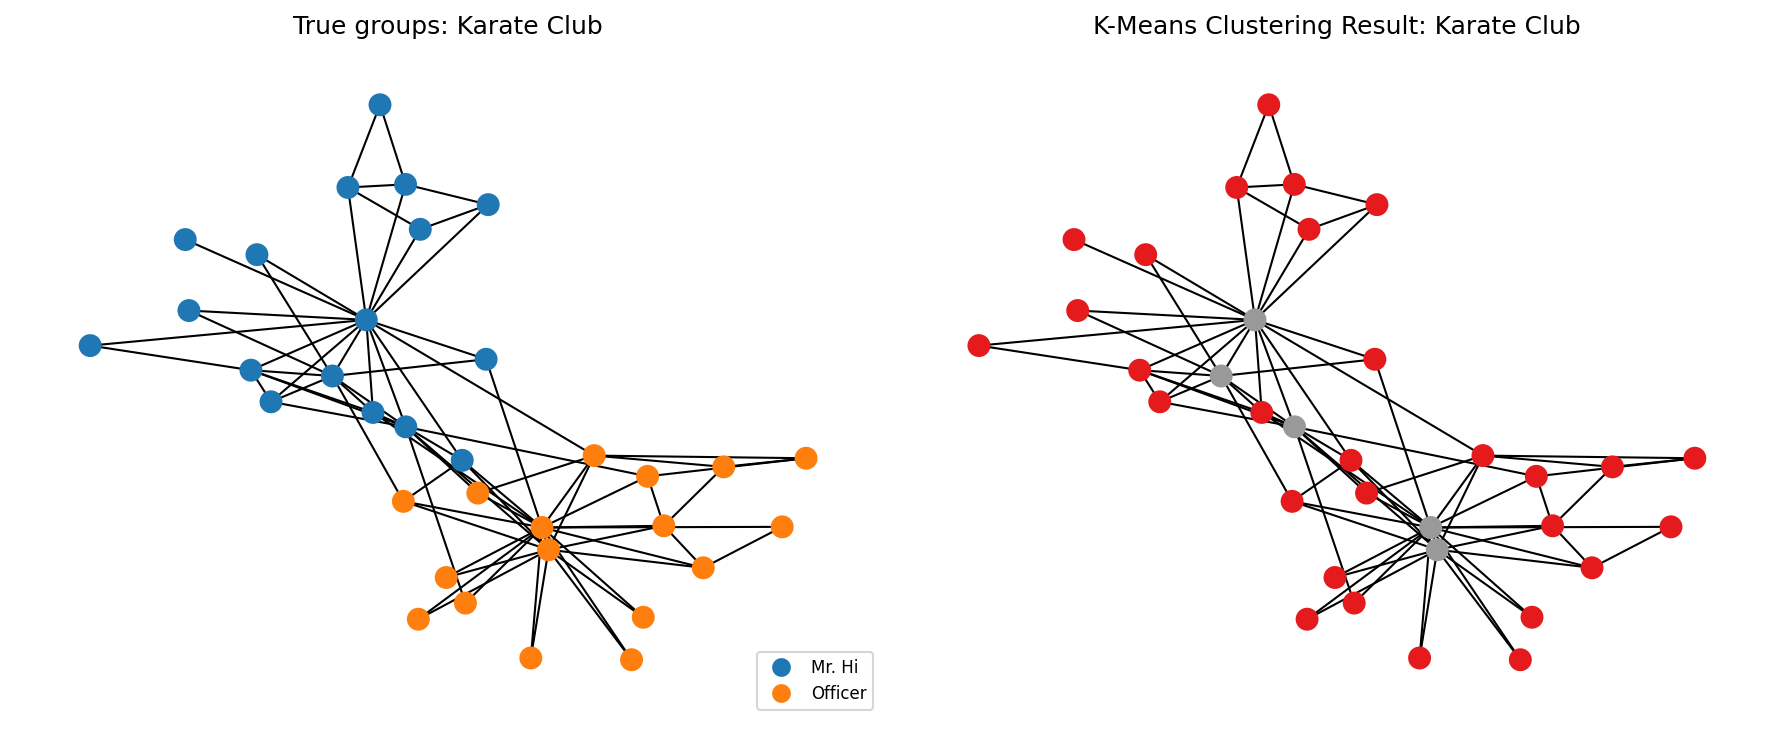
\includegraphics[width=0.5\textwidth]{output/fig2_karate_kmeans.png}
  \caption{Comparison of community detection results on the Zachary's Karate Club dataset: (Left) Ground truth division into 'Mr. Hi' and 'Officer' factions; (Right) Partition obtained using K-means clustering.}
\end{figure}

\begin{figure}[H]
  \centering
  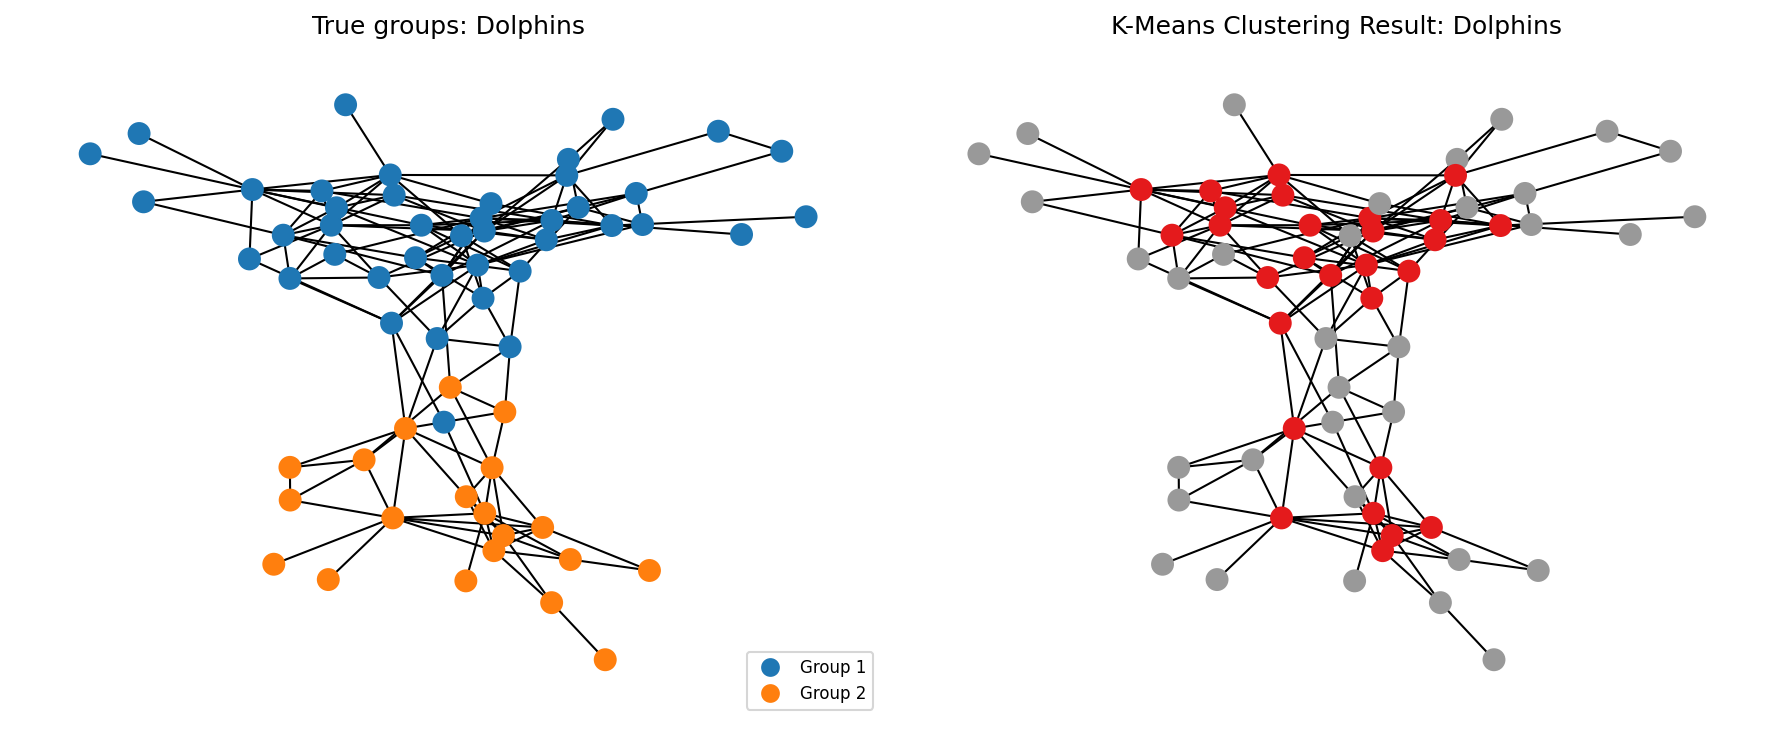
\includegraphics[width=0.5\textwidth]{output/fig3_dolphins_kmeans.png}
  \caption{Comparison of community detection results on the Dolphin Social Network dataset: (Left) Ground truth division into 'Group 1' and 'Group 2' factions; (Right) Partition obtained using K-means clustering.}
\end{figure}

\begin{figure}[H]
  \centering
  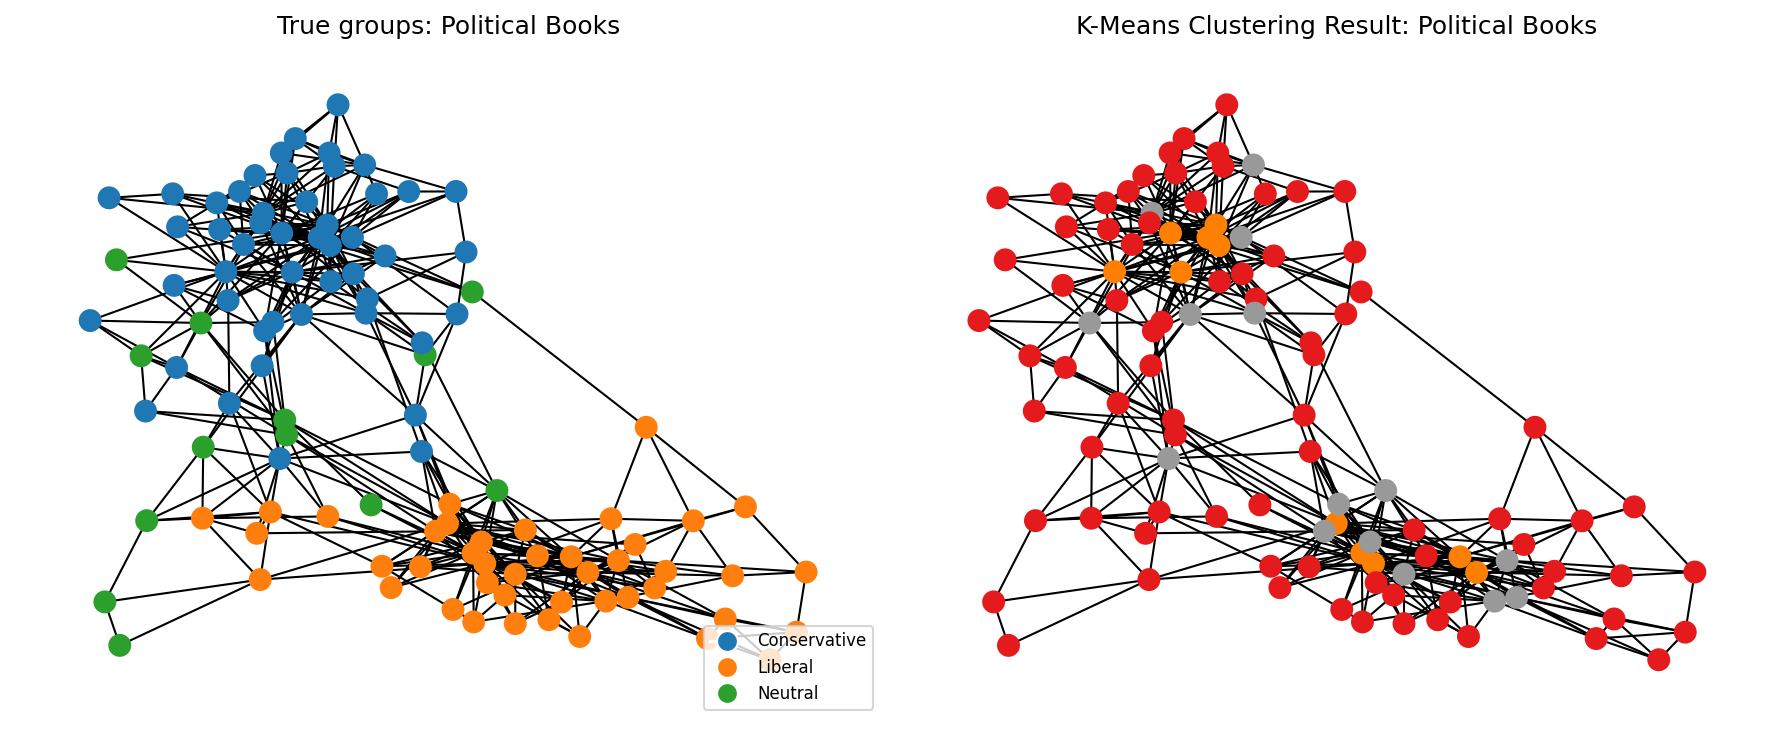
\includegraphics[width=0.5\textwidth]{output/fig4_polbooks_kmeans.png}
  \caption{Comparison of community detection results on the Books about US politics dataset: (Left) Ground truth division into 'Liberal', 'Neutral', and 'Conservative' factions; (Right) Partition obtained using K-means clustering.}
\end{figure}

\subsection{Lancichinetti's algorithm}
The visual results for Lancichinetti's algorithm is provided below where the visualization also highlights the alignment and discrepancies between the ground truth and an algorithmic output. 
This method is specifically designed to handle overlapping and complex community structures, offering a more flexible partitioning compared to traditional clustering approaches. 
In many cases, the detected communities align closely with the ground truth, though slight deviations can occur depending on the chosen resolution parameters.

\begin{figure}[H]
  \centering
  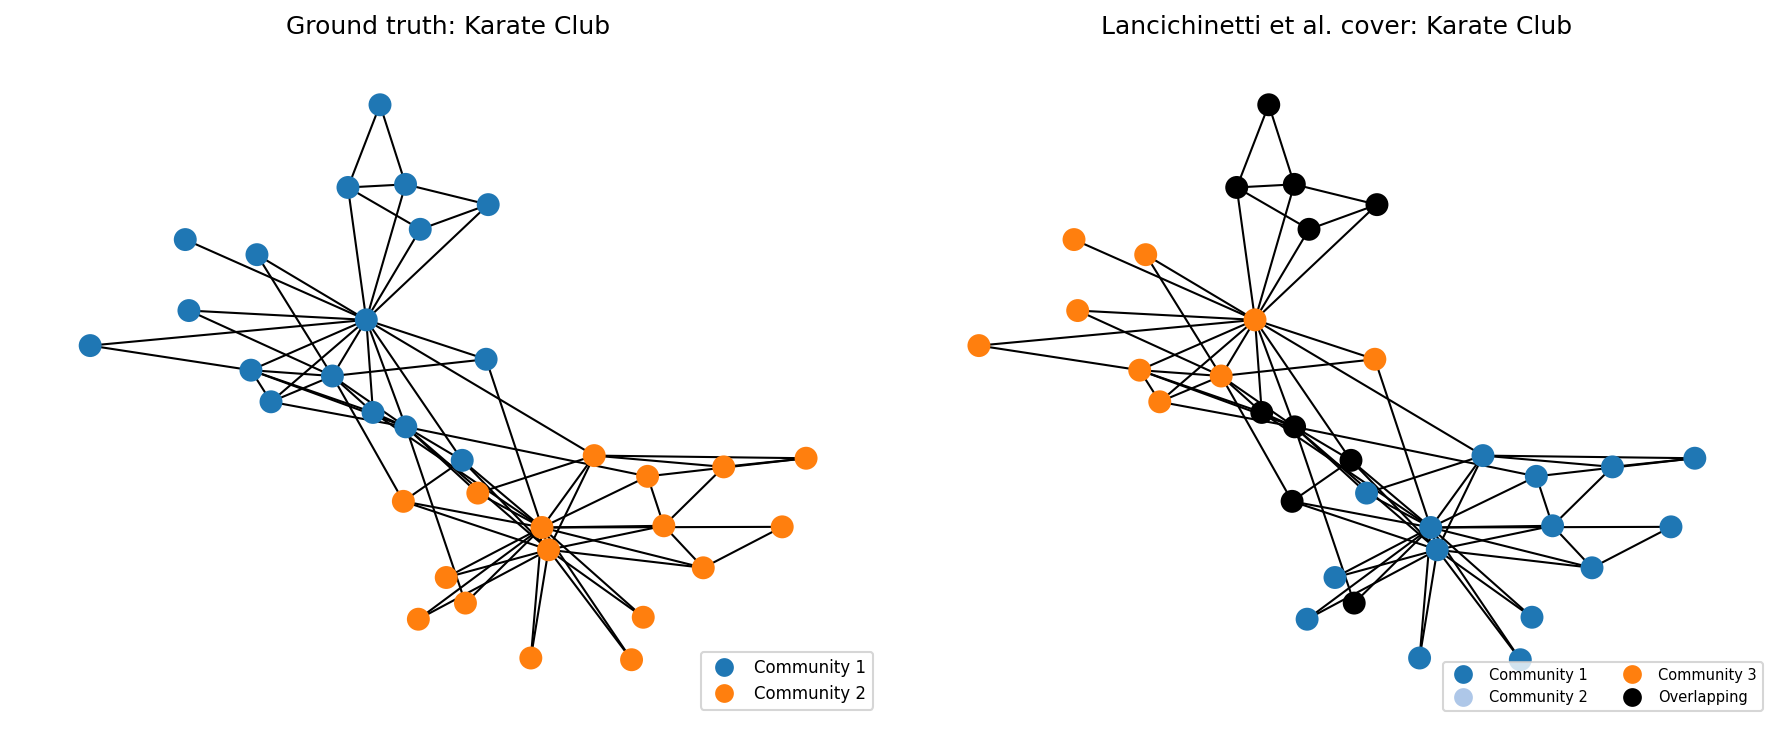
\includegraphics[width=0.5\textwidth]{output/fig6a_karate_cover.png}
  \caption{Comparison of community detection results on the Zachary's Karate Club dataset: (Left) Ground truth division into 'Mr. Hi' and 'Officer' factions; (Right) Communities detected by Lancichinetti's algorithm ($\alpha$ = 0.80).}
\end{figure}

\begin{figure}[H]
  \centering
  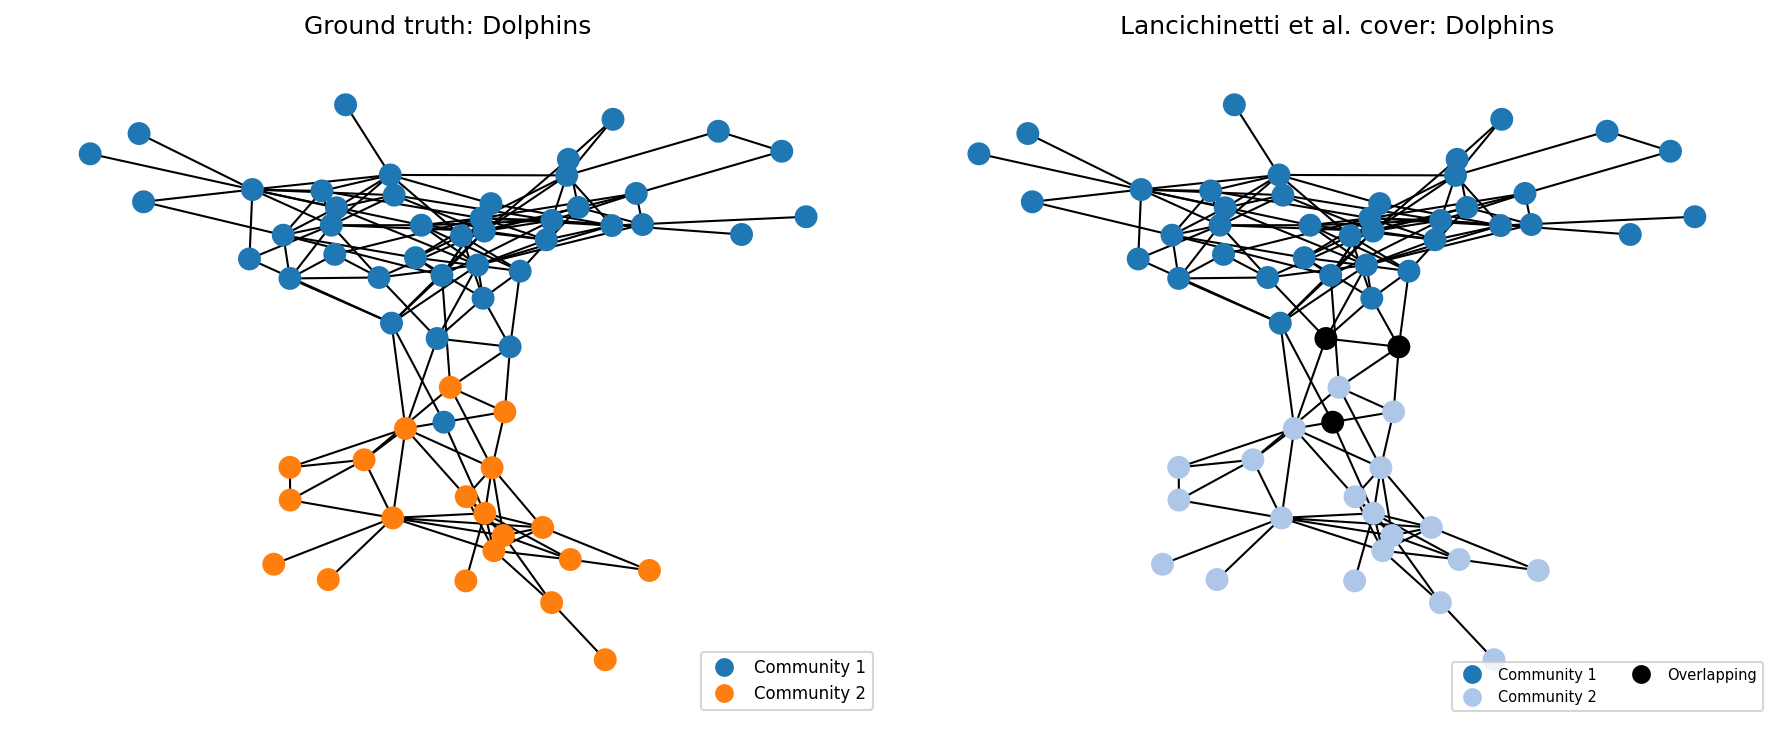
\includegraphics[width=0.5\textwidth]{output/fig6b_dolphins_cover.png}
  \caption{Comparison of community detection results on the Dolphin Social Network dataset: (Left) Ground truth division into 'Group 1' and 'Group 2' factions; (Right) Communities detected by Lancichinetti's algorithm ($\alpha$ = 0.825).}
\end{figure}

\begin{figure}
  \centering
  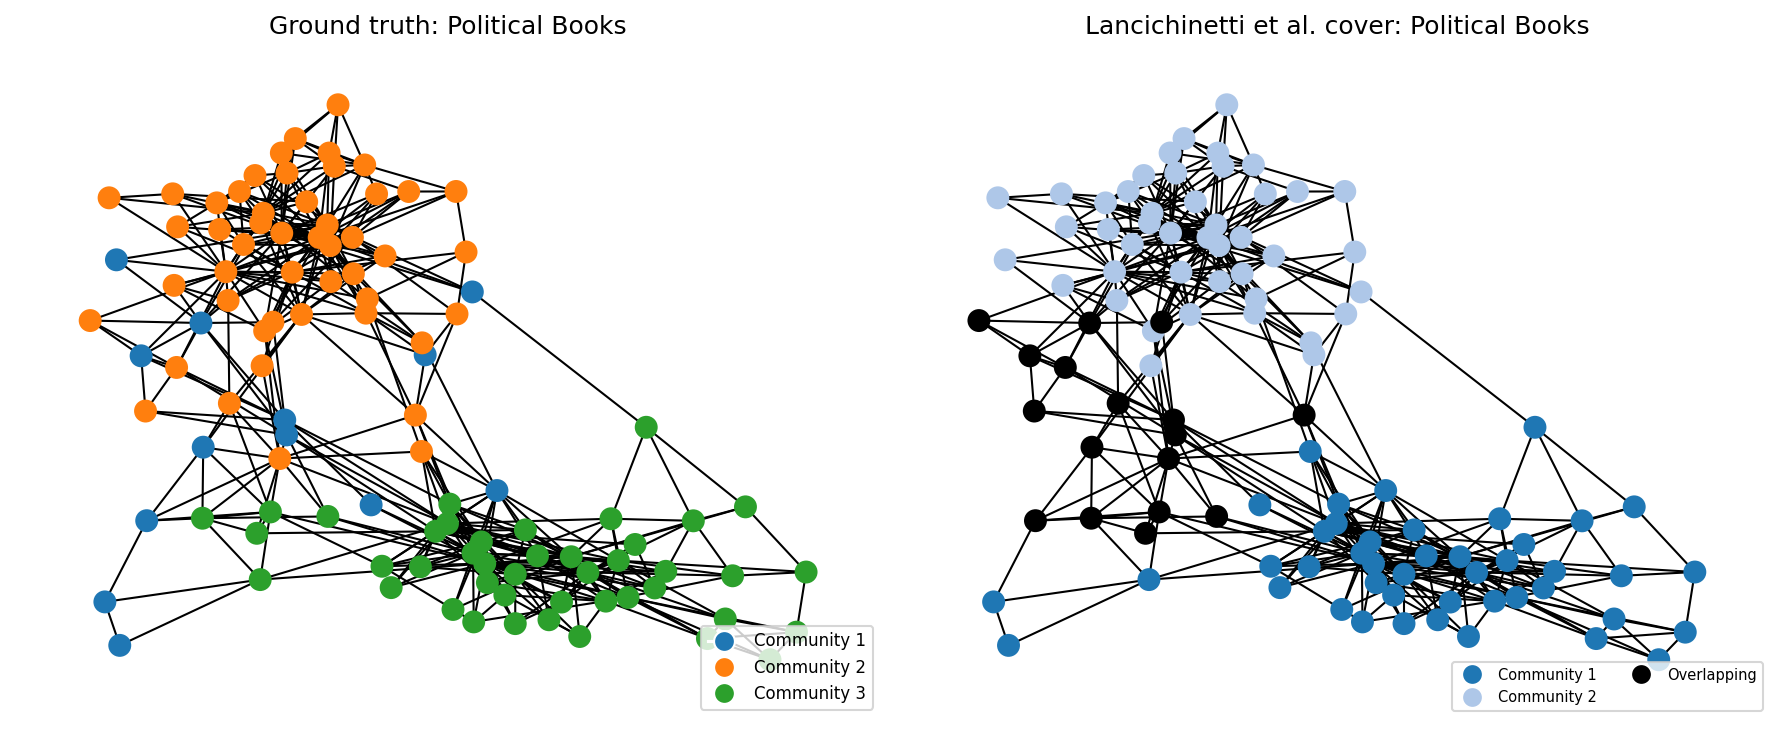
\includegraphics[width=0.5\textwidth]{output/fig6c_polbooks_cover.png}
  \caption{Comparison of community detection results on the Books about US politics dataset: (Left) Ground truth division into 'Liberal', 'Neutral', and 'Conservative' factions;(Right) Communities detected by Lancichinetti's algorithm ($\alpha$ = 0.77).}
\end{figure}
 

% ==============
% # REFERENCES #
% ==============
\bibliographystyle{IEEEtran}
\bibliography{IEEEabrv, Reference}
\end{document}